\chapter {Cell B.E. programming}
\par
In this chapter Cell B.E. platform development tools will be described as well as our experience with that tools will be mentioned.
Then particular SDK content and tools will listed.
After that parallel systems and models will be mentioned as well as the relationship to Cell B.E. development along with few design patterns.
At the end core configurations and their pros and cons will be listed finishing with some practical approaches to Cell B.E. porting process.

\section{Cell B.E. platform development}
\par
IBM deliver SDK for development of programs for Cell B.E..
It is for Linux platform, in the concrete for Fedora or Red Hat distribution.
It comes in two flavors.
The official non free one which has all the features needed for development for Cell B.E. even for some hybrid systems and support team ready to help.
And the free one that is open to wide public and everybody can download it and start developing.
The free one does not have the tools for hybrid systems nor some tools for development in other languages than C/C++.
Wee use the free one since we develop only in C/C++ and for clean Cell B.E. processor.

\par
Because the SDK is for Linux operation system, its user has to have already deeper knowledge about the system.
There are some bugs and parts that are not fully finished (see \ref{toolsSetup}).
Without deeper knowledge of the Linux system is impossible to react on some unexpected behavior during installation or development phase.

\par
We have begun with SDK version 3.0 and Fedora version 8 which ware the current version of needed tools.
We have faced some obstacles and before we were able to overcome them new version of SDK (3.1) appeared.
Because we wanted to use and describe the latest tools we had to begin from scratch because new version brought new obstacles as well.

\par
The new version was declared to be compatible with new version of Fedora (9 - Sulphur) that had been released almost some time before the new version of SDK.
Previous version of SDK (3.0) was for Fedora 7 Werewolf.
We have tried all possible combinations of Fedora distributions and SDK packages to find out if they are compatible with each other.
Only result from that was finding that the are not at the cost of lots of days spent on it.
The SDK is huge package of software dependent on lots of third party libraries and solutions.
They are treated differently within particular distributions and sometimes even versions of the same distribution.
So the result is not to combine versions (system, SDK nor particular libraries that the SDK components are dependent on.
Repository versions should be used, see \ref{toolsSetup}.

\par
Although there are to much of troubles when different version are combined, some efforts to get the SDK run on another distributions than Fedora were made.
But we thing the time spent is not worth the result.

\par
Finally we installed Fedora 9 Sulphur and SDK 3.1.
This combination is declared by IBM as tested.
Altough we have run into some bugs and errors.
The process of installation is described in \ref{toolsSetup}.
Installation of Fedora is omitted.
For details see official site \url{http://fedoraproject.org/}.

\section {SDK content}

Cell B.E. SDK is divided into variety of components.
Each component is contained in one or more rpm package for easy intallation purposes.
Here is list of most important available components:
\begin{enumerate}
  \item {Toolchain}
  \par
  Set of tools (compilers, linkers, ...) needed for actual code generation.
There are two groups of the tools.
One is for PPU and the other for SPU.

  \item {Libraries}
  \par
  IBM provides with the SDK some useful libraries for mathematics (linear algebra, FFT, Monte Carlo, ...), cryptographic or run-time management.
Code of these libraries is debugged, highly optimized for running on SPEs and SIMDized.

  \item {Full system simulator}
  \par
  Program that can simulate the Cell B.E. processor on other hardware platforms.
It is used mostly in profiling stage because simulator can simulate actual computation of a code in cycles precision.
It can of course used when programmer has not access to actual Cell B.E. hardware, but simulation is incredibly slow.

  \item {IDE}
  \par
  IDE is in fact verstion 3.2 of Eclipse with integration of debugging, profiling, Cell B.E. machine management and other features that makes development for Cell B.E. easier and more comfortable.
\end{enumerate}


\section{Parallel systems \& Cell B.E.}

Parallelization depends also on type of system (hardware) where the program will be run.
There are two basic kind of parallel systems:
\begin{enumerate}
\item {shared-memory system}
\par
Is multi-processor system with one shared memory which all processor can see.
Processors has to synchronize access to the memory otherwise race conditions will rise.

\item {distributed-memory system}
\par
Is system where each processor has its own private memory.
There is no need for synchronization.
\end{enumerate}

In context of parallel systems, Cell B.E. is some kind of hybrid system.
SPEs matches the distributed-memory system (due to private local stores) while PPE is shared-memory system.
Sometimes called heterogeneous multi-core, with distributed memory.
Because Cell B.E. processors can be gathered into bigger units (e.g. blade server, with two Cell B.E. chips) they can be viewed as either 16 + 2 cores in SMP mode or two non-uniform memory access machines connected together.
Programmer has then decide which view of the Cell B.E. processor is better for the solved problem.

\par
Because of separation of address spaces programming of SPE is very similar to client - server application design.
Roles depends on how the work is started.
In case PPU initiate the transfers the PPU is a client and SPE is a server (SPE receive some data for computation).
Another possibility that SPE grab the data from the central memory.
In this case SPE is client of central memory.
This case is preferred because the PPE is only one and would be able to manage all the SPU.

\section{Cell B.E. programming models}

\par
Implementation of parallel algorithms rely on parallel programming model.
That is a set of software technologies (such as programming languages extension, special compilers, libraries) through that actual paralelism is achieved.
So another decision that programmer has to make is to choose a programming model or mixture of them that will best fit for the solved problem.

\par
For Cell B.E. there are variety of parallel programming models.
They differ from each other in view of the hardware (hardware model) and thus how many action (such as task distribution management, data distribution management, synchronization) are performed implicitly by the model.
 The most abstract ones can perform many action implicit (i.e. ease of implementation) but at cost there can be no performance tuning done.
 And on the other hand the most concrete one see the Cell B.E. with all the details and actions performed can be tuned and performed explicitly in way application requires.

\par
There are some models that are determined only for Cell B.E. platform and are contained in SDK.
 While there are another models (such as MPI, openMP) that are compatible but they would expose only PPE, will not further described.

List of the programming models (frameworks) follows in order from most concrete to most abstract:
\begin{enumerate}
\item {libspe2}
\par
Offers features such as SPE context management (creating, running, scheduling, and deleting), DMA primitives for data transfer, mailboxes, signal, events, and synchronization functions for PPE to SPE and SPE to SPE dialogs.

\item {Data Communication and Synchronization - DaCS}
\par
Defines program entity for PPE or SPE (HE - host element program for PPE and AE - accelerator element program for SPE).
Provides some services for that programs.
These are resource and process management, where an HE manipulates its AEs.
Group management, for defining groups within which synchronization events like barriers can happen.
Message passing by using send and receive primitives etc.

\item {Accelerated Library Framework - ALF}
\par
ALF defines ALF-task as another entity that perform computationally intensive parts of a program.
The idea is to have the host program split the work into multiple independent pieces, which are called work blocks.
They are described by a computational kernel, the input and the output data. Programming with ALF is divided into two side.
The host and the accelerator one.
On the accelerator side, the programmer only has to code the computational kernel, unwrap the input data, and pack the output data when the kernel finishes.
The ALF offer clear separation between host accelerator sides of program parts.
Providing the following services (from programmers view for free): work blocks queue management, load balancing between accelerators, transparent DMA transfers, ...

\end{enumerate}

Choosing a framework is important decision of writing Cell B.E. application.
 It should be considered enough.

\section {Cell B.E. parallelism levels}

The Cell B.E. processor offers many opportunities for parallel processing.
That is because it is composed of and can be compound to heterogeneous elements.
 Levels are:
\begin{enumerate}
\item server level
\par
In a hybrid environment at the cluster level using MPI or some sort of grid computing middle-ware.

\item Cell B.E. chips level
\par
In case there are more in the machine (e.g. blade server with two Cell B.E. chips). Using ALF or DaCS for hybrid.

\item SPE level
\par
Inside the Cell B.E. chip offloading intensive parts of code to SPE, using libspe, ALF, DaCS.

\item SIMD instruction level
\par
Instruction that process more data in parallel. Using language intrinsic.
\end{enumerate}

\section{Computation configurations}

\par
Because of heterogeneous nature of Cell B.E. and its PPE \& SPEs processing elements some different computation configuration are used.
 They differ in usage of SPEs and has its own pros and cons:
\begin{enumerate}
\item Streaming configuration
\par
All SPE serves as a stream processor (see figure \ref{fg:streamingModel}).
They run exact same code expecting the same type of data and producing also the same of data type.
This configuration is well suited for some streaming application for example filters where there is still the same type of data on input.
No SPE context need not to be switched that save according time.
One disadvantage is that configuration is static.

\begin{figure}
    \centering
    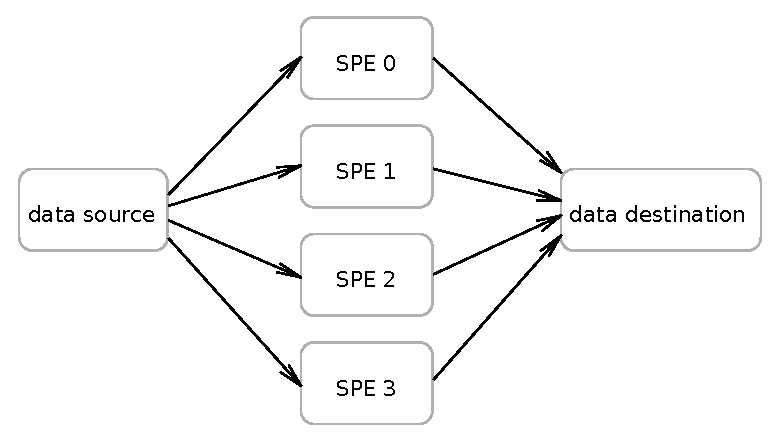
\includegraphics[width=0.9\textwidth]{data/streamingModel}
    \caption[Streaming SPE configuration]{All SPE run the same code creating farm of processor that process same type of data.}
    \label{fg:streamingModel}
\end{figure}

\item Pipeline configuration
\par
SPE server as stages of an pipeline (see figure \ref{fg:pipelineModel}).
Data are passed through from one to other of the SPEs.
The SPE to SPE transfer are faster than SPE to PPE so this can be benefit.
The configuration is also static which means no SPE context switch.

\begin{figure}
    \centering
    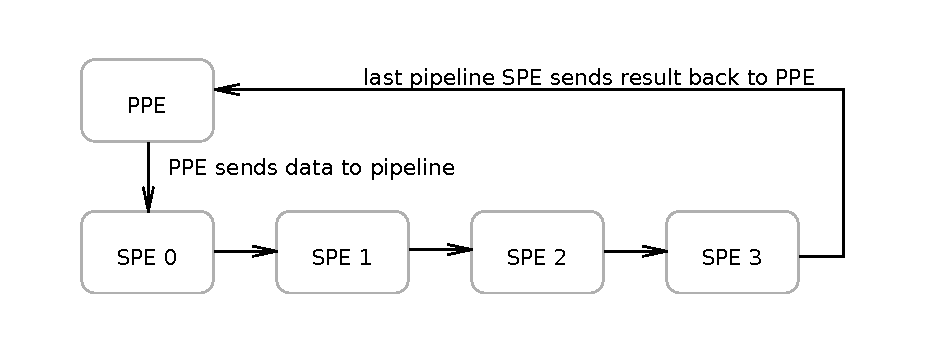
\includegraphics[width=0.9\textwidth]{data/pipelineModel}
    \caption[Pipeline SPE configuration]{SPE creates pipeline. Each SPE represent one stage of that pipeline. Data are transferred only via SPE to SPE DMA transfers benefiting the speed of bus.}
    \label{fg:pipelineModel}
\end{figure}

\item PPE centric
\par
This configuration is common approach with Cell B.E..
Program runs on PPE (see figure \ref{fg:PPUCentricModel})and only selected, highly demanding computational kernels (hotspots) are offloaded to SPEs.
This method is the easiest from a program development perspective because it limits the scope of source code changes and does not require much re-engineering at the application logic level.
One disadvantage is dynamic changes of SPE contexts that is quite expensive opertation.

\begin{figure}
    \centering
    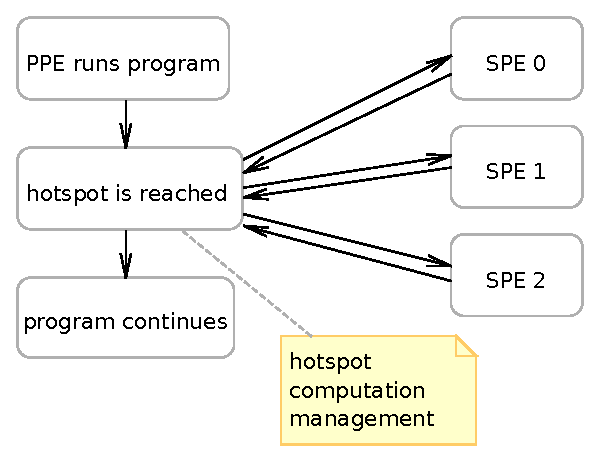
\includegraphics[width=0.7\textwidth]{data/PPUCentricModel}
    \caption[PPU centric configuration]{Program is run on PPE and only hotspots are offloaded to SPEs.
 Offloading means managing SPE context creation and loading as well as managing data transfer and synchronization between PPE and SPEs}
    \label{fg:PPUCentricModel}
\end{figure}

\item SPE server
\par
Another configuration is to have server-like programs running on SPEs that sits and waits offering some functionality.
 This is requires the code to be small enough to fit into the SPU local store along with processed data.

\end{enumerate}

\section {Building for Cell B.E.}
\par
Actual compilation process is performed using appropriate tool chain.
PPE code using of PPE tool chain and SPE code using SPE one.
But there is difference between management of code in linking stage between PPU and SPU object files.
It is caused by difference of actual code usage.
While PPU code resides in central memory (just like in common architectures) SPU code is loaded into SPE dynamically and shall be somehow separated.
It is similar to shader programs for graphic accelerators.
They are also loaded into appropriate processors when they are needed so they live separated (in form of files).

\par
There are two options for SPE code management.
 One is to build shared library and load it explicitly when it is used.
Another way is to build a static library and include it into PPU executable using Cell B.E. Embedded SPE Object Format (CESOF).
This allows PPE executable objects to contain SPE executables i.e. SPE binary is contained within PPE binary. See figure\ref{fg:SPEEmbedding}.
This inclusion is called embedding and is performed with extra tool from tool chain.
The SPU program is then referenced as special external structure direct from PPU code (instead of performing some shared libraries loading).
Both ways has its pros but even cons which are the same as with shared vs. static libraries on other platforms.


\begin{figure}
    \centering
    
\includegraphics[width=0.8\textwidth]{data/SPEEmbedding}
    \caption[SPE binary embedding]{Illustration how is SPE binary 'embedded' into a PPE binary.
SPE binary is another section of PPE binary.
It is reachable through extern struct variable, that contains pointer to SPE binary.}
    \label{fg:SPEEmbedding}
\end{figure}



\section {Process of porting application for Cell B.E.}
\label{sect:portingProcess}

Common process of porting an application for Cell B.E. processor (figure \ref{fg:appPorting}).
\begin{enumerate}
\item Hotspots localization
\par
Through profiling of the application on PPE we find most compute intensive parts, hotspots.

\item Hotspots porting for SPE
\par
Hotspot code is then moved to the SPEs.
This mean adaptation the code for SPE (DMA transfers instead of direct memory access, appropriate data structures, etc.).
Data movement tuning (using different data structures) can be performed until satisfactory performance is obtained.
\end{enumerate}

Following steps are necessary for application optimization and speed-up.
They increase utilization of all the SPU features that means whole register set utilization, dual-issue of instructions, SIMD execution and DMA transfers.
More detail in \cite{writingPerfApps} part 4:
\begin{enumerate}
\item{Multi-buffering}
\par
Data that resides within central memory and are processed by SPE should be copied onto local store buffer before actual computation.
When there are more these buffers program can take advantage from asynchronous DMA transfer and process current buffer while next data are transferred to another buffer.
Then the buffers are simply swapped and SPU need not to wait until transfer of next data is complete (see figure \ref{fg:multibuffering} for detail).

\begin{figure}
    \centering
    \includegraphics[width=0.5\textwidth]{data/multibuffering}
    \caption[Multi-buffering]{Difference between arrays of structure and structure of arrays}
    \label{fg:multibuffering}
\end{figure}

\item{Branch elimination}
\par
Elimination of branches elongates instruction chain where no branch is performed.
In such chain all data always go through the same instructions that makes possible to perform SIMDation.
This step brings more advantage because branching is problem for every processor.
Branch elimination is probabbly the most complicated step of the porting process.

\item{SIMDation}
\par
Rewriting scalar code into vectorized to be able to use SIMD instruction.
In this step the most performance gain could be achieved because of multiple data processing by one instruction.
But it is conditioned by well performed the previous step.
This is because when SIMD instruction are used every single piece of data should go through the exactly same order of instructions.
The most important method of this step is arrays of structure to structure of arrays conversion.
The Figure \ref{fg:simdation} shall illustrate this method.

\begin{figure}
    \centering
    \includegraphics[width=0.5\textwidth]{data/SIMDation}
    \caption[SIMDation]{Difference between arrays of structure and structure of arrays}
    \label{fg:simdation}
\end{figure}

\item{Loop unrolling}
Means putting more loop bodies serially into code.
This decrease loop count and elongate the loop body.
Example:
\begin{verbatim}
for(uint32 i=0; i<32; i++)
{
    std::cout << ".";
}
\end{verbatim}
become (by loop unrolling with factor 2)
\begin{verbatim}
for(uint32 i=0; i<16; i++)
{
    std::cout << ".";
    std::cout << ".";
}
\end{verbatim}
This is positive for compiler that can do more optimizations (better instruction scheduling and register utilization).

\item{Instruction scheduling}
\par
Proper reorganization of instructions can give us some more performance in some cases.
This step is performed by the compiler but can be performed manually in assembly language.

\item{Branch hinting}
\par
Give the processor hint what result will be after future branch.
It is done through insertion of special instructions.
This step should be again performed by the compiler but can be performed manually in assembly language.

The whole process is repeated for every single hotspot.
\end{enumerate}

\begin{figure}
    \centering
    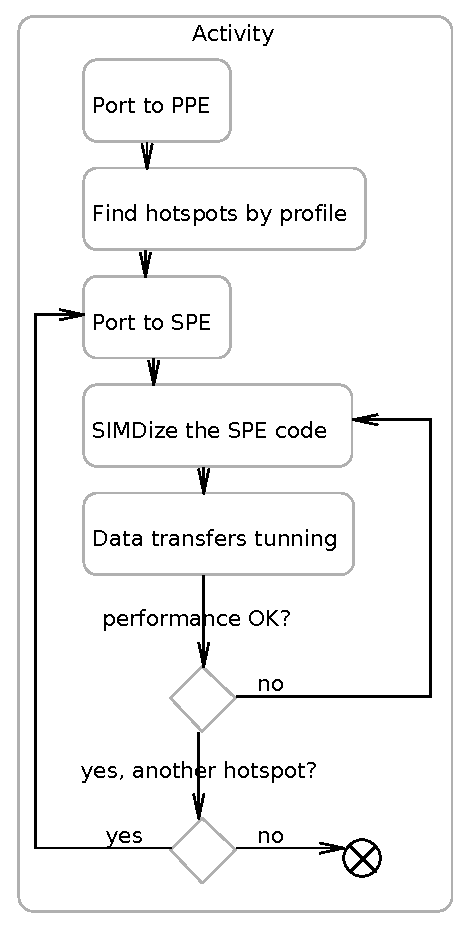
\includegraphics[width=0.5\textwidth]{data/portingCycle}
    \caption[Application for Cell B.E. porting process]{Diagram shows all stages of the process and loops for better performance tuning and other hotspots}
    \label{fg:appPorting}
\end{figure}

\section {SPE porting considerations}

\par
Main SPE feature that everything spin around while porting code to SPE is local store size.
On the one side are decisions about data transfers.
This means how the data that has to be processed by the SPE will be transferred into local store and vice versa.
What will be the sizes of data chunks.
How many buffers will be used in case of multi-buffering.
On the other side is code complexity of the solved problem that influence the size of final binary (alternative is SPE overlays, run-time download program kernels).
All these things has programmer take into consideration to make the final binary smaller than local store.
Everything is big tradeoff between processed data chunk sizes with number of buffers of that chunks and code complexity (how large algorithm can be).
\par
When compiling the SPU binary from ported code the final executable will probably increase the local store size.
Even when the code seems not as large as the final binary size.
Then begins big searching what causes this huge size.
We have gone through some problems with code that is common in non SPE code but cause problems in SPE code.
Here is the list:
\begin{enumerate}
\item usage of keyword new
\par
There is no memory allocation on SPE. So new is meaningless.
But compiler accepts it without any complain.

\item usage of std streams
\par
This code:
\begin{verbatim}
#include <iostream>
std::cout << "Hallo" << std::endl;
\end{verbatim}
goes through the compiler without complaints but makes the final binary to big.

\end{enumerate}

\section {Speed and compiler options}

\par
There is variety of compiler options.
Usage of some of them is worth nothing but can increase performance and avoid some kind of bugs.

\par
Mike Acton explains in \cite{strictAliasing} the strict aliasing and its impact for performance.
Another advantage to let this checked by the compiler is fact that it can avoid bugs that would appear as far as in release stage when optimizations flags are used in compilation.
In this stage is this kind of bugs really hard to track and debug.

\par
Another option advises are in \cite{compilerOptions}